\chapter{Integrated Circuits}
\label{kap:hardware}
Typical electronic circuits are made of different electronic components, such as resistors, capacitors and transistors. Building them up in a discrete way needs much space and so those devices are miniaturized and built up on one semiconductor plate to an IC. In that way, millions of transistors can be placed on a chip of the size of some cm$^2$. The miniaturization of electronic circuits gives some important advantages:
\begin{itemize}
\item low size: thousands of transistors can be placed on one chip;
\item low power dissipation: Due to smaller component sizes the energy usage is lower and so less power is dissipated by heat;
\item high processing speed due to short wiring length; and
\item low costs due to mass production. Several ICs can be manufactured on one waver plate in one production process.
\end{itemize}
\section{Power consumption of ICs}
In digital systems the power consumption plays an important role. Especially in mobile or space systems where the amount of available energy is limited, the power usage of the system should be analyzed. As the power consumption depends on frequency and supply voltage, decreasing any of them is advantageous. Due to less heat dissipation, stress gradients associated to heat are decreased. Furthermore the limited power on mobile or space devices can be used more efficiently.\\
Digital systems need both dynamic and static power, where the whole power demand is calculated as
\begin{equation}
P=P_{static}+P_{dynamic}\;.
\end{equation}
\subsection{Static power consumption}
Generally CMOS devices have a low static power consumption. This consumption occurs when no states are changed and when they are constant. Static power consumption occurs due to reverse-bias leakage between diffused regions and the substrate.\cite{Sar97} With improving manufacturing technologies, the gate thicknesses decrease and consequently the probability for tunneling effects increases. For this reason, leakage currents are increasing with increasing technologies.\cite{Iye10} The total leakage current between the supply voltage $V_{DD}$ and ground can be determined by
\begin{equation}
P_{static}=I_{DD}\cdot V_{DD}\;.
\end{equation}
\subsection{Dynamic power consumption}
Every wire and logic gate has capacitive effects. When an IC switches from one state to another state, those capacities have to be charged. The energy to charge from 0 to the supply voltage $V_{DD}$ can be determined by $C\cdot V_{DD}^2$. When the capacities are discharged from $V_{DD}$ to 0, no power from the supply is used\cite{Har13}, therefore discharging does not have to be modelled for power considerations. Assuming the IC to be clocked with frequency $f$, there are $\frac{f}{2}$ charging processes as well as $\frac{f}{2}$ discharging processes per second. In this way, the maximum dynamic power can be calculated by
\begin{equation}
P_{dynamic}=\frac{f}{2}\cdot C\cdot V_{DD}^2\;.
\end{equation}
\subsection{Observations on power consumption}
As the total power consumption of an IC can be seen as $P=V_{DD}*\big(I_{DD}+\frac{1}{2}\cdot f\cdot C\cdot V_{DD}\big)$, the consumption can be lowered when decreasing the supply voltage $V_{DD}$ and the frequency $f$. For correct operation of semiconductor devices like transistors and diodes, the threshold voltage has to be exceeded, so the supply voltage can not be decreased boundlessly. Therefore the exact need of calculation speed should be observed in advance, and in that way the clock rate of ICs should be set to the lowest possible frequency which is well adapted for reasonable operation. 
\section{IC types}
Generally ICs can be subdivided in two groups. If they are used for different purposes like microprocessors, they are called \textit{general purpose IC}. Otherwise if they are used only for specific applications they are \textit{application specific ICs}. ASICs and FPGAs are typical types of application-specific chips.
\subsection{Microprocessor}
Microprocessors are built up as general purpose processors to compute a whole set of commands called machine language. The machine code then is a long sequence of operations. For executing a program the operation code (opcode) is fetched into the instruction register. The address for the next opcode is stored in the program counter. A microprocessor contains mainly following blocks as shown in figure \ref{fig:microprocessorblockdiagram}:
\begin{itemize}
\item Arithmetical Logical Unit (ALU)\\
This block is the central unit of the processor. Using control inputs a lot of arithmetical and logical operations can be done. As the ALU does not contain any memory cells, operation registers have to store the data as long as the operation is finished. Most ALUs are not able to compute all operations (e.g. multiplications), so those operations have to be done using other operation codes (a multiplication can be done using shift and add-operations). 
\item Instruction Register (IR)
\item Program Counter (PC)
\item Registers\\
Registers are a set of flipflops grouped together with a single command. Each flipflop is able to store one bit. For more information on flipflops see chapter \ref{ch:flipflops}. All microprocessors have a whole set of registers, some of them can be seen external. Those can be used to read data from the bus or write data to the data bus. Accessing registers is much faster than using memory chips. This is due to the higher clock rate of processors than the bus system. Furthermore the address decoder as well as the bus interface have not to be activated for the access.\\
While some registers can be used for different purposes some special registers are built up for some special usage. Such special registers are memory control registers or the accumulator. 
\item Control Unit\\
This block is used for decoding the opcodes and coordinating all other blocks. As some operations need access to the bus system the control unit has to do complex sequences of signals in a exact defined time lapse. Furthermore interrupts and other command signals have to be computed. A simple and approved method to do this is using special ROM components.\cite{Wue06}\\
A simplified procedure of the control unit can be given as
\begin{enumerate}
\item load PC to the address bus
\item set the external control signals to read-access on the memory
\item read the opcode from the data bus and store it to the IR
\item decode the opcode
\item increment the PC
\end{enumerate}
Item 1 to 3 are called \textit{instruction read cycle}.
\item Memory Controller\\
For addressing and read/write-access to the data and address bus the memory controller is used. Typical addressing schemes are direct memory access, register indexed addressing, indexed access as well as memory indirect addressing.
\item Bus system\\
The components of a microprocessor are connected using buses. Information is exchanged using those bus system. Typically the bus system contains 3 buses, subdivided by functionality:\cite{Bei04}
\begin{itemize}
\item The \textit{address bus} is used for target and source adresses of data transmissions.
\item The \textit{data bus} is used for data transfer.
\item The \textit{internal bus}, often also called \textit{control bus}, is used for coordinating the data transfer in means of direction and sequence of the data transfer.
\end{itemize}
\end{itemize}
\begin{figure}[htbp]
\begin{center}
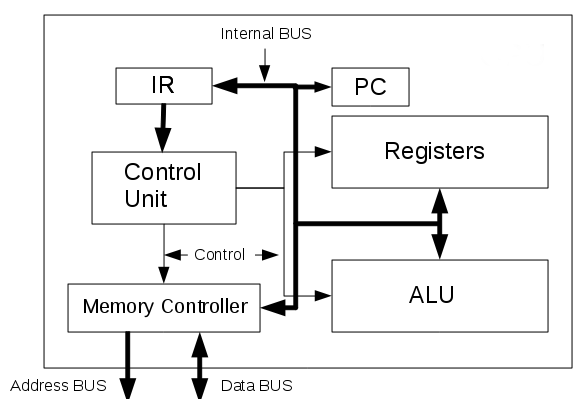
\includegraphics[width=10cm,keepaspectratio=true]{bilder/png/microprocessorblockdiagram}
\caption{Internal structure of a microprocessor}
\label{fig:microprocessorblockdiagram}
\end{center}
\end{figure}
\subsection{ASIC - Application Specific Integrated Circuit}
ASICs are ICs which are designed for a specific purpose. Examples for those ICs are control systems for washing machines, graphic card accelerators or network interface chips. ASICs are typically faster than FPGAs or multi purpose processors as they are specialized for one specific usage and the chip are is very low compared to other types. But as disadvantage manufacturing is expensive, because the masks for the waver production have to be made for every single chip design. In that way the manufacturing process for ASICs is only suitable for mass production, where one chip design is used for thousands of devices.
\subsection{FPGA - Field-Programmable Gate Array}
In comparison to ASICs the FPGA can be programmed for different applications after delivery. The programming is done by combining a large number of logic blocks (CLB, LAB) and lookup tables (LUTs) through configurable bus connections. As FPGAs are reprogrammable, a design change in very late design phases is possible, even over remote connections. A general structure of a FPGA can be seen in figure \ref{fig:fpgablocksgeneral}. A FPGA is programmed using a HDL (see section \ref{kap:HDL}).
\begin{figure}[htbp]
\begin{center}
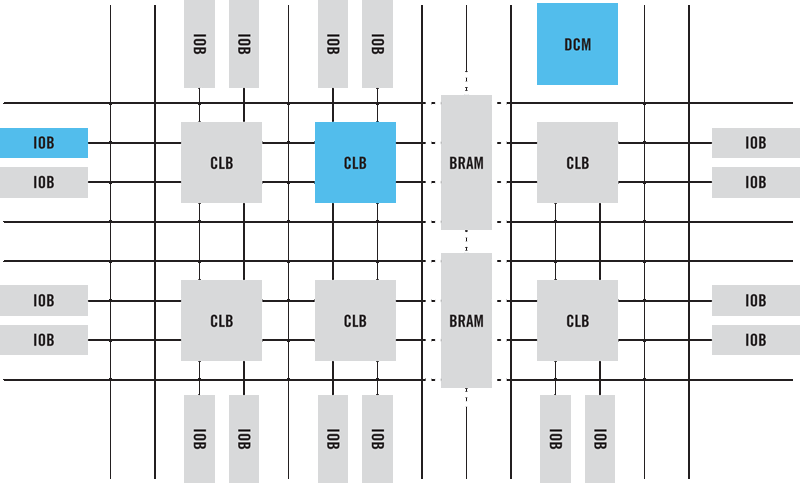
\includegraphics[width=14cm,keepaspectratio=true]{bilder/png/fpgablocksgeneral}
\caption{Internal design of FPGAs}
\label{fig:fpgablocksgeneral}
\end{center}
\end{figure}
\subsubsection{SRAM-based devices}
The most common FPGA type is SRAM-based. SRAM cells are typically made of 4 to 6 MOSFET transistors (but also special factoring types with up to 10 transistors exist). The transistors are connected as bistable flipflops to store each bit. A typical SRAM cell is shown in figure \ref{fig:SRAMaufbau}. So those devices are volatile and have to be programmed each time they are powered up. As they can be programmed further and further again they are suitable for prototyping and updating the configuration. As disadvantages it has to be mentioned that SRAM-based devices are more sensitive to radiation and therefore they need additional shielding. Furthermore, due to the physical design they need more space and so less space for logic arrays is available.\cite{Maxfield2009}\\
\begin{figure}[htbp]
\begin{center}
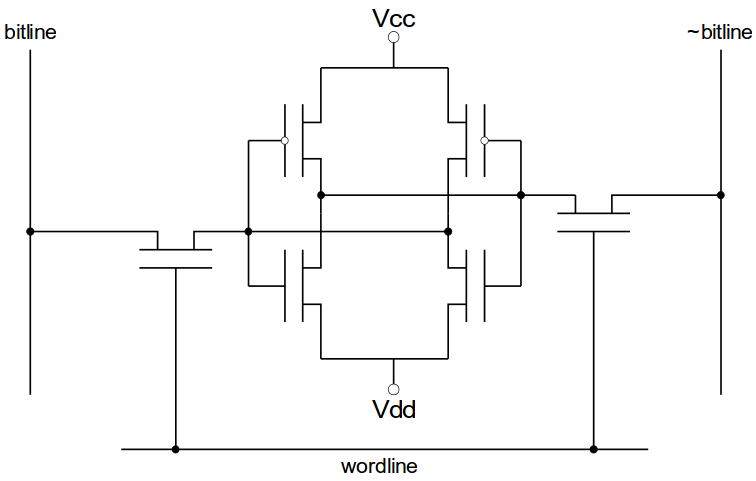
\includegraphics[width=8cm,keepaspectratio=true]{bilder/png/SRAMaufbau}
\caption{Design of a SRAM memory cell\cite{Core16}}
\label{fig:SRAMaufbau}
\end{center}
\end{figure}
\subsubsection{Antifuse-based devices}
Antifuse-based devices are OTP. The programming is done with special programming devices. For manufacturing those devices special materials, eg. non-conducting amorphous silicon, are used.\cite{Zeif2011} When antifuse-based devices are programmed, conducting channels are made by high voltage. This can be seen in figure \ref{fig:antifusevorhernachher}. So when antifuse-based FPGAs are programmed the configuration is permanent. This leads to the fact that the configuration of the device is non-volatile and available at power-on. The configuration can be hidden due to special security antifuses. Due to the fact that the device is OTP, no additional memory is needed to store the configuration. The disadvantage of this device is that it can be programmed only once and so it is not suitable for prototyping or changing configurations. Furthermore the programming can only be done off-line.\\
Antifuse-based configurations are radiation hard and therefore suitable for military or space environments.\cite{Maxfield2009} It must be pointed out, that only the configuration is naturally radiation hard, and attached components have to be made radiation hard (shielding, TRD) as well. As antifuses need more manufacturing steps than SRAM-based devices, antifuse-based devices are some technology generations behind.
\begin{figure}[htbp]
\begin{center}
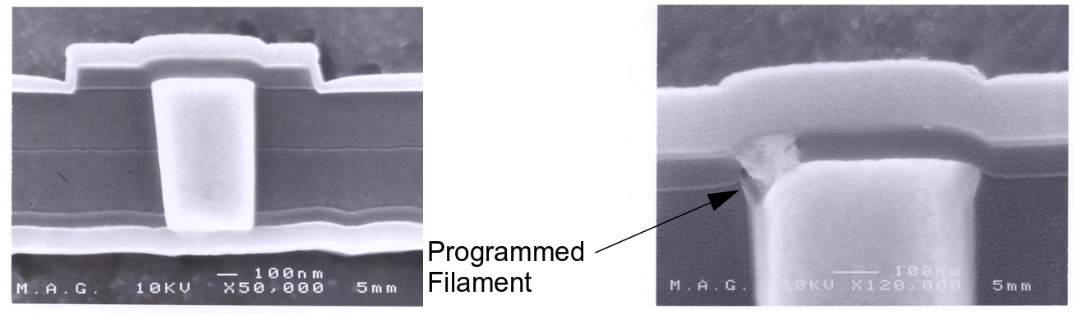
\includegraphics[width=10cm,keepaspectratio=true]{bilder/png/antifusevorhernachher}
\caption{An unprogrammed (left) vs programmed (right) antifuse cell \cite{Qui16}}
\label{fig:antifusevorhernachher}
\end{center}
\end{figure}
\subsubsection{Flash-based devices}
Flash-based devices can be electrically programmed and erased, so that they can be configured over and over again. This can be done offline or online via special programming interfaces (in-circuit programmable). The memory is non-volatile and so the configuration can be stored even after power-off. As disadvantages the relatively high static power consumption\cite{Qui16} as well as device altering due to programming cycles have to bementioned. Flash-based devices contain a large number of flash-cells, which use two floating-gate transistors for storing data. A floating-gate transistor can be seen in figure \ref{fig:FlashTransistor}\\
\textit{The floating-gate is isolated, insulated all around by an oxide layer, with no electrical contacts. This means that any electrons placed on the floating-gate are literally trapped until removed. This persistence is the foundation for using flash memory as storage.}\cite{Flash16}\\
A detailed description of the operating of floating-gate transistors can be found at \cite{Cse16}.\\

\begin{figure}[htbp]
\begin{center}
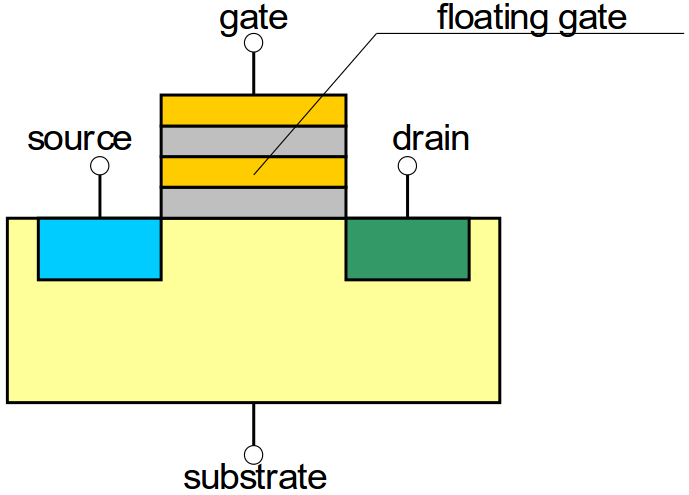
\includegraphics[width=7cm,keepaspectratio=true]{bilder/png/FlashTransistor}
\caption{A floating-gate transistor used in flash memory\cite{Core16}}
\label{fig:FlashTransistor}
\end{center}
\end{figure}
\section{Hardware elements}
In this section some important hardware elements are explained.
\subsection{Flip-flops}
\label{ch:flipflops}
Flipflops are basic logic elements with 2 stable states. They consist of a data input and a clock input, as well as a data output. Optionally a set/reset-pin or an inverted output can be available. Fliipflops are used as memory elements. Simplified, a logical state at the data input is stored at the rising edge of the clock signal, and held stable to the output until the next rising edge occures. The most used flipflop is the D-flipflop.
\begin{figure}
\begin{center}
    \subfigure[RS-flipflop]{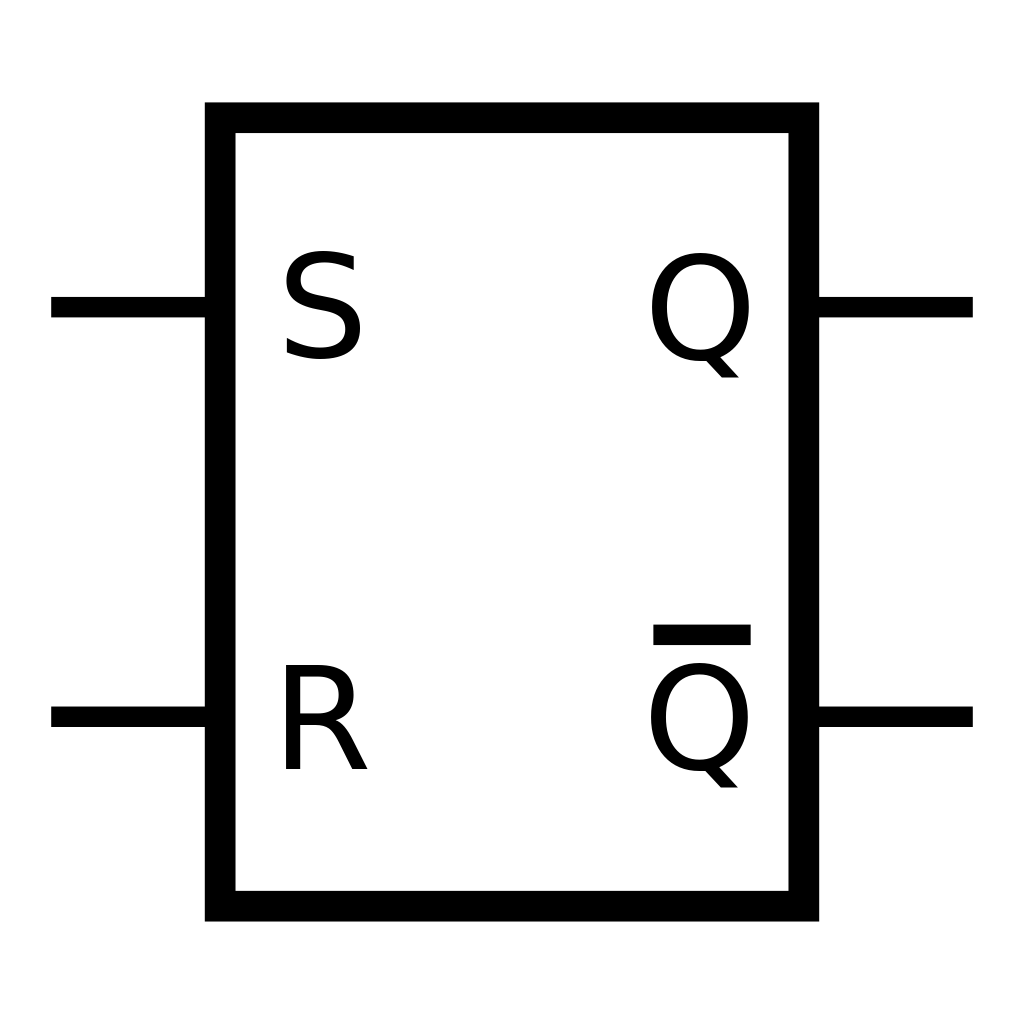
\includegraphics[width=2.5cm,keepaspectratio=true]{bilder/png/RSflipflop}\label{fig:rsflipflop}}
    \subfigure[JK-flipflop]{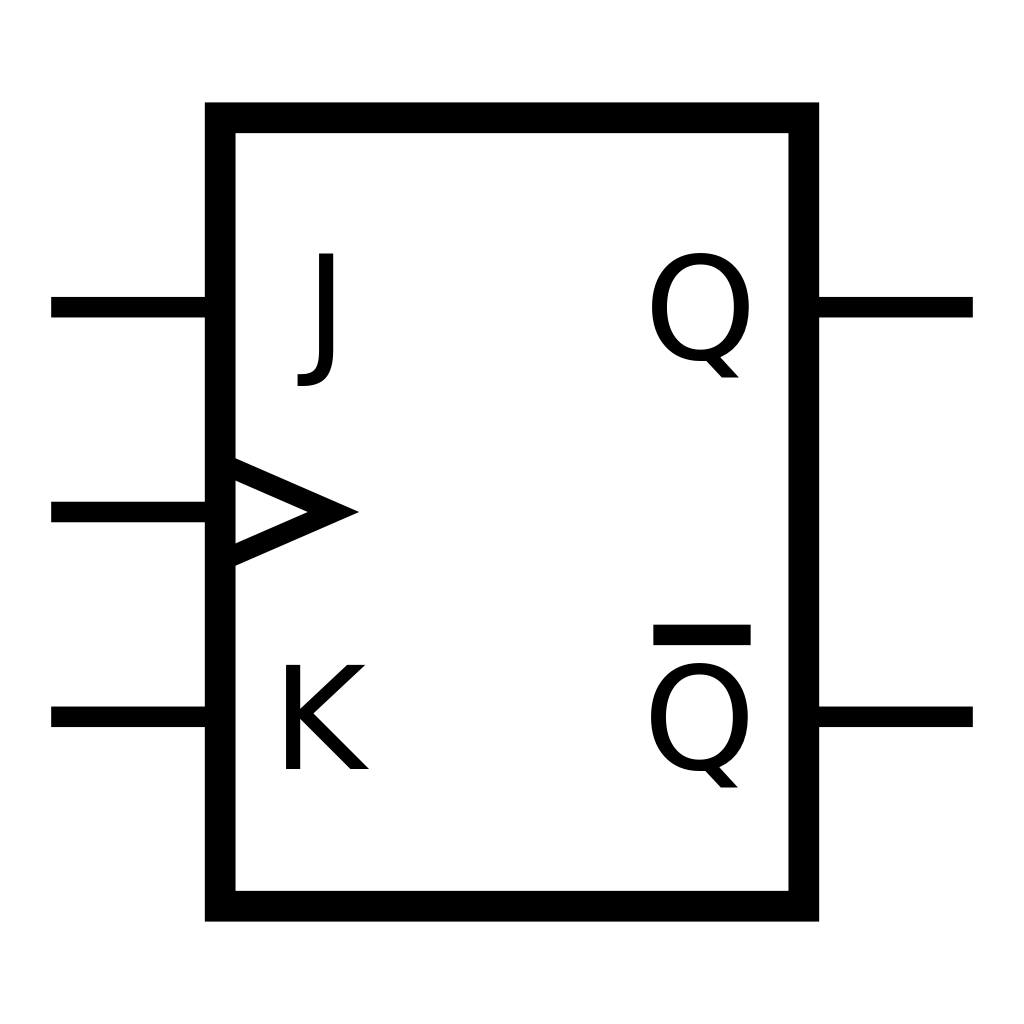
\includegraphics[width=2.5cm,keepaspectratio=true]{bilder/png/JKflipflop}\label{fig:jkflipflop}}
    \subfigure[T-flipflop]{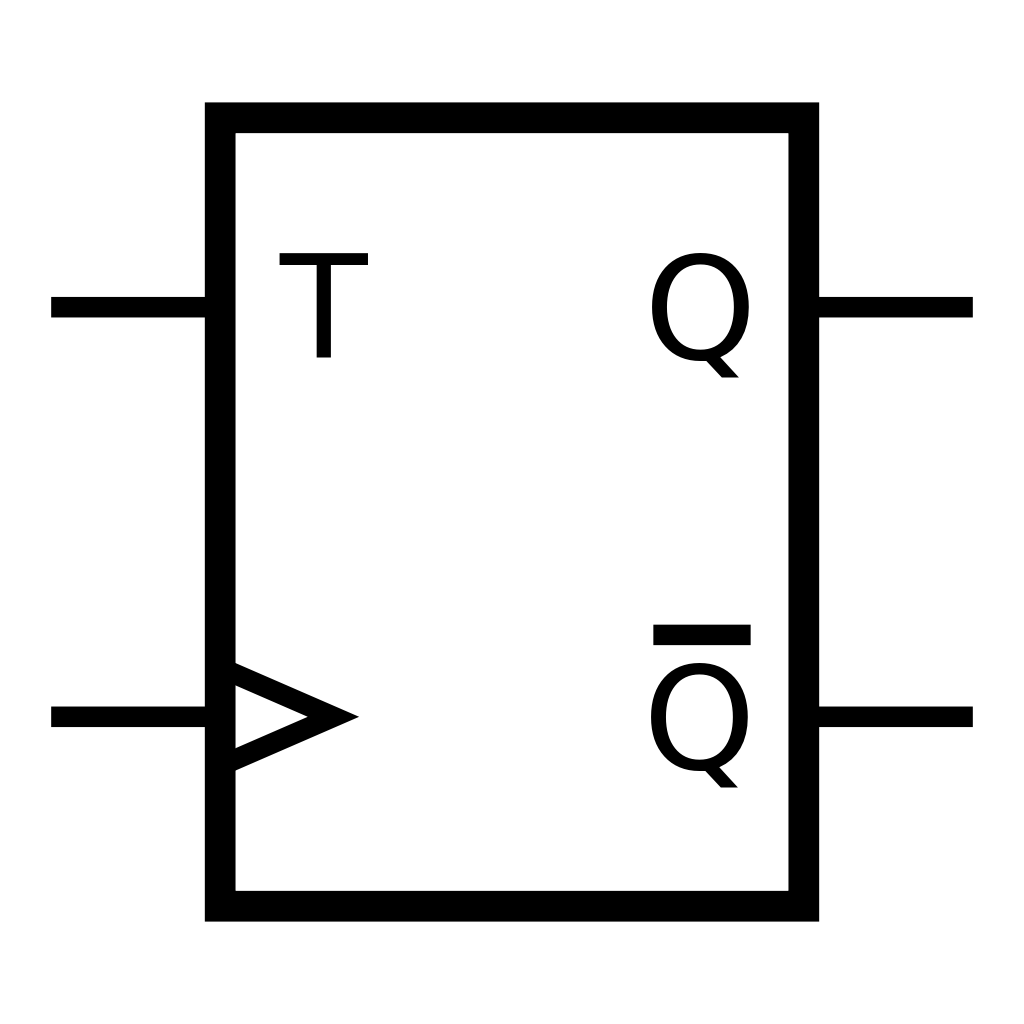
\includegraphics[width=2.5cm,keepaspectratio=true]{bilder/png/Tflipflop}\label{fig:tflipflop}}
    \subfigure[D-flipflop]{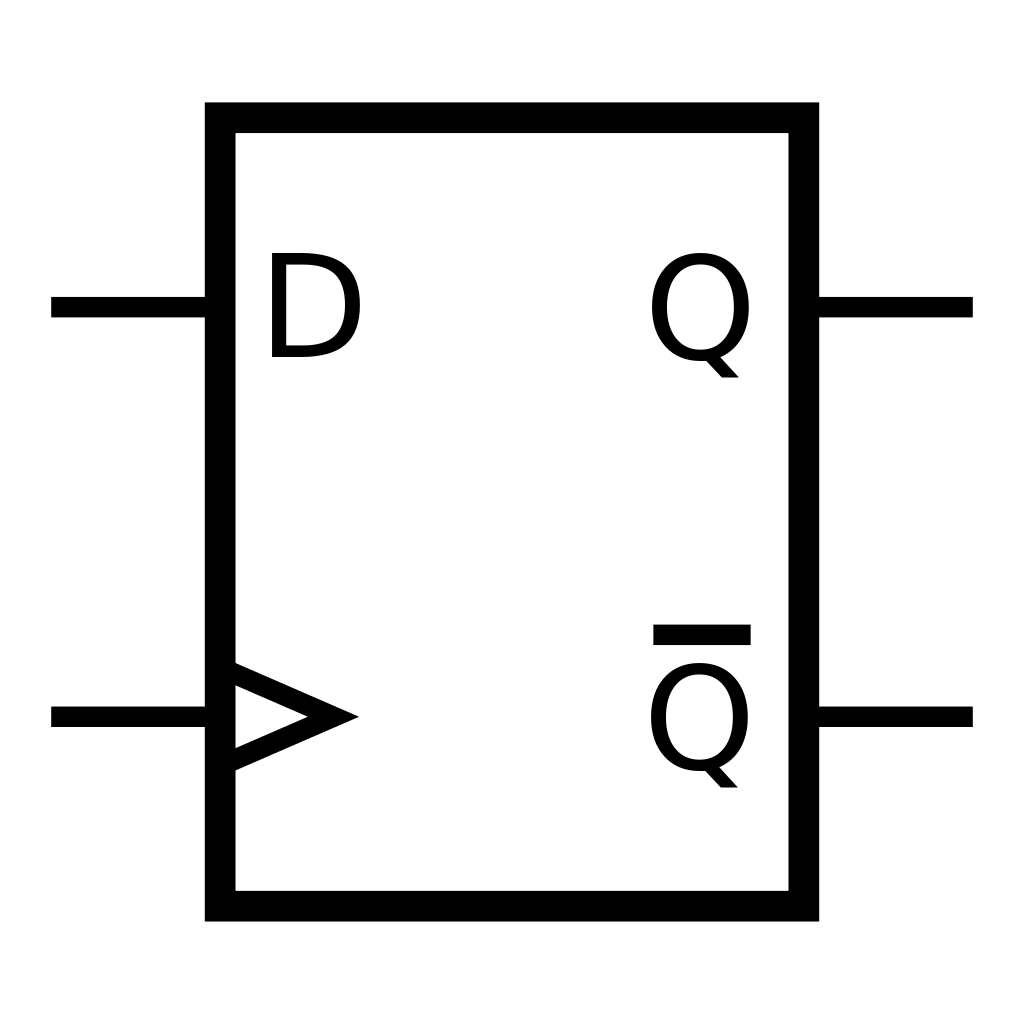
\includegraphics[width=2.5cm,keepaspectratio=true]{bilder/png/Dflipflop}\label{fig:dflipflop}}   
\caption{logic blocks of different flipflop types}
\end{center}
\end{figure}

\begin{itemize}
\item RS-flipflop\\
The RS-flipflop, which can be seen in figure \ref{fig:rsflipflop}, is the most simple form of a flipflop. It consists of a set and a reset input. The state change is asynchrously and therefore not depending on rising clock edges. 

\begin{table}
\begin{center}
\begin{tabular}{|c|c||c|}
\hline
S &  R & $Q_{t+1}$\\
\hline\hline
0 & 0 & $Q_{t}$\\
\hline
0 & 1 & 0\\
\hline
1 & 0 & 1\\
\hline
1 & 1 & undefined\\
\hline
\end{tabular}
\caption{Input/Output states of a RS-flipflop}
\label{tab:rsstates}
\end{center}
\end{table}

The different state transitions of a RS-flipflop are listed in table \ref{tab:rsstates}. As long as the R and S bits are set to low state the output is held constant at the previous state. When the reset bit is set the output is changed to 0, when the set bit is set to 1, Q changes to 1. When R as well as S are both set, the output is simultaneously forced to get low and high. In this metastable state the next state is undefined and is dependent on factoring characterizations.

\item RES-flipflop\\
In addition to the simple RS-flipflop this type has an enable input. This causes state changes to only occur when the enable bit is set. The advantage of this configuration is that state changes due to inconsistencies on the input lines. Even though the RES-flipflop has an enable pin it is still an asynchronous device.
\item JK-flipflop\\
The JK-flipflop (shown in figure \ref{fig:jkflipflop} is like a universal flipflop. It can be configured as RS-flipflop D-flipflop as well as a T-flipflop. The state transitions can be found in table \ref{tab:jkstates}. The transitions are like the RS transitions, but as difference the J=K=1 state is interpreted as toggle state.

\begin{table}
\begin{center}
\begin{tabular}{|c|c||c|}
\hline
J &  K & $Q_{t+1}$\\
\hline\hline
0 & 0 & $Q_{t}$\\
\hline
0 & 1 & 0\\
\hline
1 & 0 & 1\\
\hline
1 & 1 & toggle\\
\hline
\end{tabular}
\caption{Input/Output states of a JK-flipflop}
\label{tab:jkstates}
\end{center}
\end{table}

\item T-flipflop\\
The T-flipflop as shown in figure \ref{fig:tflipflop} performs no state transition as long as the T-input is set low. When it is set to 1 the flipflop starts to toggle, the next state will be set to the inverse of the current state, corresponding to the clock rate. The state transitions are listed in table \ref{tab:tstates}.
\begin{table}
\begin{center}
\begin{tabular}{|c||c|}
\hline
T & $Q_{t+1}$\\
\hline\hline
0  & $Q_{t}$\\
\hline
1  & $\overline{Q_{t}}$\\
\hline
\end{tabular}
\caption{Input/Output states of a T-flipflop}
\label{tab:tstates}
\end{center}
\end{table}

\item D-flipflop\\
The D-flipflop is the most used flipflop.It can be seen in figure \ref{fig:dflipflop}. The D-flipflop reads the D input at the rising edge of the clock and is therefore a synchronous device. The output is set to the D input at the rising edge and held stable at any other time. In this way the D-flipflop can be seen as simple memory cell

\end{itemize}

\subsubsection{Timing properties}
When using flip-flops some timing parameters are important (seen in figure \ref{fig:flipfloptiming}) and explained below.
\begin{itemize}
\item setup time $t_{S}$\\
The setup time is the time the input signal has to be hold constant before the rising clock of the edge occurs to sample the input reliable, using synchronous devices.
\item hold time $t_{H}$\\
THe hold time is the duration the input signal has to be hold stable after the rising clock edge occured for a reliable input sampling. $t_{H}$ is a property of synchronous flipflops.
\item recovery time\\
The recovery time is like $t_{S}$ for asynchronous flipflops. This is applied, because not every short signal change should have impact on the output. 
\item removal time\\
The removal time is like the hold time for asynchronous devices.
\item propagation delay $t_{P}$, $t_{CO}$\\
The propagation delay is the time the flipflop needs to change the output state after the rising clock edge occured. In some cases the delay times for low-to-high transition is not equal the high-to-low transition time. The propagation delay times are denoted in the datasheets. For correct operation of the flipflop the clock time has to be lower than $t_{S}+t_{H}$.
\end{itemize}
\subsection{Clock}
In this part some possibilities to generate the clock signal are explained.
\paragraph{Resonant circuit\\}
The most simple form of generating an oscillating signal is a circuit consisting of a capacitor, inductor and resistor. It oscillates due to the interaction of the magnetic field of the inductor and the electric field of the capacitor. When the capacitor is charged, current flows through the inductor building up a magnetic field. As the capacitor will be decharged the voltage decreases. The magnetic field is a maximum when the capacitor voltage reaches 0. Now the capacitor will start to charge with negative current increasing the electric field while the magnetic field decreases. The circuit starts to oscillate according to Faraday's law. The natural frequency of the oscillation can be determined using
\begin{equation}
f_0=2\pi\omega_0
\end{equation}
with
\begin{equation}
\omega_0=\frac{1}{\sqrt{LC}}
\end{equation}
RLC-circuits are used in many different applications, eg. for tuning radios or as frequency filters. The disadvantages of this type of resonator are the relatively low Q-factor and the fact that resonance frequency is not stable to temperature changes.
\paragraph{Crystal oscillator\\}
One of the most important things of oscillators is frequency stability. High stability referring to temperature or changes in the supply voltages is given using quartz crystals. A quartz crystal is a silicon oxide with defined shape and size. Both sides are metallized. When a voltage is applied, a piezo-electric effect occurs and the generated mechanical force leads to electrical charges. As the physical shape can not be changed after production, the frequency stays constant and is inverse proportional to the thickness of the crystal. The symbol of crystal oscillators in electric circuits is shown in figure \ref{fig:crystaloscillatorsymbol}.
\begin{figure}[htbp]
\begin{center}
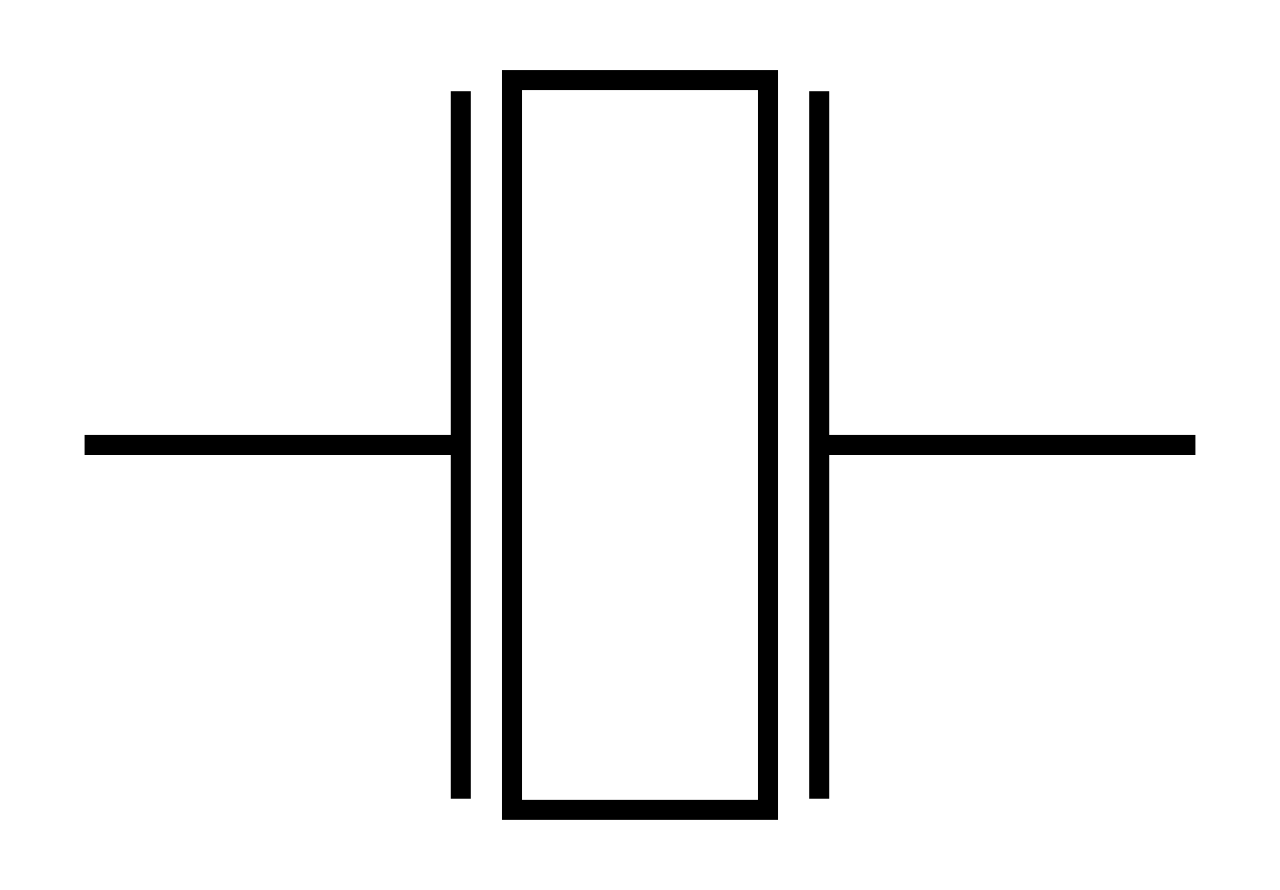
\includegraphics[width=1cm,keepaspectratio=true]{bilder/png/crystaloscillatorsymbol}
\caption{IEC symbol of an oscillator}
\label{fig:crystaloscillatorsymbol}
\end{center}
\end{figure}
\paragraph{Phase-locked loop\\}
A PLL is a system, which allows a signal to stay constant to an external reference clock. A block diagram of a PLL is shown in figure \ref{fig:pllblocks}. As reference clock most times a crystal oscillator is used. The reference clock signal is divided and the phase of this reference signal is compared with the output of the PLL. What the PLL now does is to keep the phase between the two signals constant (as it can be seen in figure \ref{fig:pllphase}). For this the error signal, given by the phase comparator, is lead to a VCO . This signal is divided by another divider and fed back to the phase comparator.\\
In comparison to other oscillators with variable frequency the long term stability is very high. The dividers can be changed very quickly and so frequency changes can be realized easily. Furthermore the divider values can be configured digitally and so remote modification is possible. As disadvantages higher phase noise and the complexity of the systems have to be mentioned.
\begin{figure}[htbp]
\begin{center}
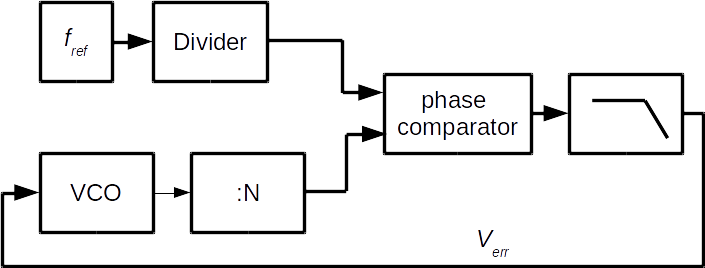
\includegraphics[width=12cm,keepaspectratio=true]{bilder/png/PLLblocks}
\caption{Block diagram of a PLL}
\label{fig:pllblocks}
\end{center}
\end{figure}
\begin{figure}[htbp]
\begin{center}
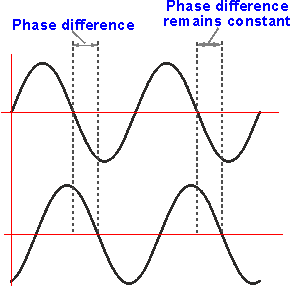
\includegraphics[width=6cm,keepaspectratio=true]{bilder/png/PLLphase}
\caption{Phase diagram of a PLL}
\label{fig:pllphase}
\end{center}
\end{figure}